\documentclass[12pt]{article}
% \usepackage{titling}
\usepackage[utf8]{inputenc}
\usepackage[english]{babel}
\usepackage[12pt]{extsizes}
\usepackage{graphicx}
\usepackage{tikz}
\usepackage{tikz-feynman}
\usepackage{float}

\usepackage{authblk}

% \usepackage{titlesec}
\usepackage{amsthm,amsfonts,amsmath,amssymb,amscd, amsbsy}  % AMS (American Mathematical Society) mathematical extensions

\usepackage{url}
\usepackage{listings}
% \usepackage{cleveref}
\newcommand{\abs}[1]{\lvert#1\rvert}
% \titlelabel{\thetitle.\quad}
\usepackage{geometry}
\geometry{a4paper,top=2.0cm,bottom=2.0cm,left=3.0cm,right=1.5cm,footskip=4mm}
% \setlength{\oddsidemargin}{0cm} % Adjust this value to control the left margin
% \setlength{\textwidth}{17cm}

% \setlength{\droptitle}

\title{Implementation Errors of Model 1 (Background: Poisson, Efficiency: Binomial) in TRolke}
\date{}
% \pagenumbering{gobble}

\author[1]{Yu. Maslov\thanks{y.maslov@g.nsu.ru}}
\author[2]{D. Maximov \thanks{D.A.Maksimov@inp.nsk.su}}
\affil[1]{Novosibirsk State University, Novosibirsk, Russia}
\affil[2]{Budker Institute of Nuclear Physics, Novosibirsk, Russia}

\begin{document}
\maketitle{}
\vspace{-5em}

\section{Introduction}
In \cite{Rolke_paper}, a method for constructing confidence intervals using the profile likelihood approach is described.
This method was implemented in the TRolke (ROOT class) for several models of signal-detection efficiency and background, which, despite being considered legacy and obsolete at present, continues to be used.
Section 2.2 of \cite{Rolke_paper} states that the system of equations for finding the suprema required to construct intervals in the model (denoted in TRolke as model 1)
$$X\sim \mathrm{Pois}(\epsilon \mu +b),\qquad Y\sim \mathrm{Pois}(\tau b),\qquad Z\sim \mathrm{Bin}(m,\epsilon)$$
(where $\mathrm{Pois}$ denotes the Poisson distribution and $\mathrm{Bin}$ denotes the binomial distribution)
cannot be solved analytically and must be solved numerically; this statement is incorrect.
During the implementation of the numerical solution of this system, a number of errors were also made.

This note presents an analytic solution of the aforementioned system and an implementation of this solution. A comparison is performed between the likelihood suprema obtained with the original implementation (containing an error) and those obtained with the corrected analytic approach.
It is shown that the analytic implementation yields larger values over a set of parameters than the suprema produced by the original method.

In addition, the analytic solutions for the remaining models were verified; no errors in solving the equations or in implementing the supremum search were found.

\section{Existence of an Analytic Solution}

In the profile likelihood method for constructing confidence intervals, the following statistic is used:
$$\lambda \left(\mathbf{\pi}_0 | X\right) = \frac{\sup\left\{ L \left(\mathbf{\pi}_0, \mathbf{\theta } | X\right); \mathbf{\theta } \right\} } {\sup\left\{ L \left(\mathbf{\pi}, \mathbf{\theta } | X\right); \mathbf{\pi}, \mathbf{\theta } \right\}} ,$$
where $\mathbf{\theta }$ are nuisance parameters.

In model 1, the background is modeled by a Poisson distribution, and the efficiency by a binomial distribution:
$$L(\mu, b, \epsilon | x, y, z, m, \tau) = \frac{\left(\epsilon \mu + b\right)^x}{x!} e^{-\left(\epsilon \mu + b\right)} \frac{\left(\tau b\right)^y}{y!} e^{-\left(\tau b\right)} C_m^z \epsilon^z \left(1 - \epsilon\right)^{m-z} ,$$
$$\ln L(\mu, b, \epsilon | x, y, z, m, \tau) = $$
$$ = x\ln \left(\epsilon \mu + b\right) -\left(\epsilon \mu + b\right) + y\ln \left(\tau b\right) - \tau b + z \ln \epsilon + \left(m - z\right) \ln \left(1 - \epsilon\right) + C ,$$
where $C$ denotes the contribution from the factorials and the binomial coefficient.
To find an extremum, one must solve the system of equations obtained by setting the partial derivatives with respect to the nuisance parameters equal to zero.
In \cite{Rolke_paper}, the following system of nonlinear equations is given, together with the statement that no analytic solution can be obtained:
\begin{equation*}
    \frac{\partial }{\partial b}\log l(\mu ,b,\epsilon|x,y,z)=\frac{x}{\epsilon\mu +b}-1+\frac{%
    y}{b}-\tau \doteq 0
\end{equation*}
    
\begin{equation*}
    \frac{\partial }{\partial \epsilon}\log l(\mu ,b,\epsilon|x,y,z)=\frac{x}{\epsilon\mu +b}-\mu +%
    \frac{z}{\epsilon}-\frac{m-z}{1-\epsilon}\doteq 0 .
\end{equation*}

It should be noted that the system above contains a typo: the factor $\mu$ was dropped when differentiating with respect to $\epsilon$. The correct system is:
\begin{equation} \label{partial_b_eq}
    \frac{\partial }{\partial b}\log l(\mu ,b,\epsilon|x,y,z)=\frac{x}{\epsilon\mu +b}-1+\frac{%
    y}{b}-\tau \doteq 0
\end{equation}
    
\begin{equation} \label{partial_eff_eq}
    \frac{\partial }{\partial \epsilon}\log l(\mu ,b,\epsilon|x,y,z)=\frac{x \mu}{\epsilon\mu +b}-\mu +%
    \frac{z}{\epsilon}-\frac{m-z}{1-\epsilon}\doteq 0 .
\end{equation}

Contrary to the statement in \cite{Rolke_paper}, this system can be solved analytically by reducing it to a quartic equation and applying standard methods for solving 4th-degree polynomials.
From \eqref{partial_b_eq}, it follows that
$$\epsilon \mu + b = \frac{x}{1 + \tau - \frac{y}{b}} \Rightarrow \epsilon = \frac{1}{\mu} \left(\frac{x}{1 + \tau - \frac{y}{b}} - b\right) = \frac{b}{\mu} \left( \frac{x - b \left(1 + \tau\right) + y}{b \left(1 + \tau \right) - y}\right) .$$
Introduce the following notation: $R(b) = x + y - b \left(1 + \tau\right)$, $Q(b) = b \left(1 + \tau\right) - y$. Hence, $\epsilon = \frac{b}{\mu} \frac{R(b)}{Q(b)}$.
Next, multiplying \eqref{partial_b_eq} by $\mu$ and subtracting it from \eqref{partial_eff_eq}, we obtain:
$$\left(\tau - \frac{y}{b}\right) \mu + \frac{z}{\epsilon} - \frac{m - z}{1 - \epsilon} = 0 \Rightarrow \left(\tau - \frac{y}{b}\right) \mu + z\frac{\mu Q(b)}{b R(b)} - \frac{m - z}{1 - \frac{b}{\mu} \frac{R(b)}{Q(b)}} = 0 .$$
Introduce one more notation, $S(b) = \mu Q(b) - b R(b)$. Then:

\begin{equation}
\begin{split}
      1 - \frac{b}{\mu} \frac{R(b)}{Q(b)} = \frac{\mu Q(b) - b R(b)}{\mu Q(b)} = \frac{S(b)}{\mu Q(b)} \Rightarrow \\
       \left(\tau - \frac{y}{b}\right) \mu + z\frac{\mu Q(b)}{b R(b)} - \left(m -z\right) \frac{\mu Q(b)}{S(b)} = 0 .
\end{split}
\end{equation}

Multiply this equation by $b R(b) S(b)$. Then:
$$\left(\tau b - y \right) \mu R(b) S(b) + z \mu Q(b)S(b) - (m-z) \mu b Q(b) R(b) = 0 .$$

It can be seen that this equation is a 4th-degree polynomial, which can be solved analytically in the general case.
This equation can be brought to the form
$A b^4 + B b^3 + C b^2 + D b + E =0$, where:
$$A = - \mu \tau \left(1 + \tau\right)^2 ,$$
$$B = \mu (1+\tau) (m (1+\tau)-\mu \tau (1+\tau)+2 \tau x+y+3 \tau y) ,$$ 
$$C = \mu(-m (1+\tau) (x+2 y)-(x+y) (\tau x+2 y+3 \tau y)+\mu (1+\tau) (y+z+\tau (x+3 y+z))) ,$$
$$D = \mu y \left(m (x+y)+(x+y)^2-\mu (x+2 \tau x+2 y+3 \tau y+2 (1+\tau) z)\right) ,$$
$$E = \mu^2 y^2 (x + y + z) .$$


\section{Error in the Implementation of the Numerical Solution}

Due to the statement that the system of equations \eqref{partial_b_eq}, \eqref{partial_eff_eq} is not analytically solvable, the following algorithm for finding the suprema was implemented in TRolke \cite{TRolke, ROOT}:
instead of reducing the system to a single equation, the total derivative with respect to $\epsilon$ is set to zero (this derivative is computed by the LikeGradMod1 class method) using the bisection method (the bisection is implemented in the ProfLikeMod1 class method):
$$\frac{d \ln f}{d \epsilon} = \frac{x}{\epsilon \mu + b} \left(\mu + b^\prime\right) -  \left(\mu + b^\prime\right) + \frac{y}{b} b^\prime - \tau b^\prime + \frac{z}{\epsilon} - \frac{m -z}{1 - \epsilon} = 0 .$$
Further, from the original system of equations \eqref{partial_b_eq}, \eqref{partial_eff_eq} it follows that
$$-\frac{y \mu}{b} +\tau \mu = \frac{m-z}{1-\epsilon} - \frac{z}{\epsilon} .$$
Let $\eta = \frac{z}{\epsilon} - \frac{m-z}{1-\epsilon}$, $\eta^\prime = - \frac{z}{\epsilon^2} - \frac{m-z}{\left(1-\epsilon\right)^2}$. Then
$$-\frac{y}{b} +\tau = - \frac{\eta}{\mu} \Rightarrow b = \frac{y}{\tau + \eta / \mu} \Rightarrow  b^\prime = - \frac{b^2}{y \mu} \eta^\prime .$$

However, in the technical implementation of this relation in the TRolke class, shown in Fig.~\ref{fig:code_with_error}, the following expressions for $b$ and $b^{\prime}$ are used:
$$b = \frac{y}{\tau - \eta / \mu} , \hspace{1.5cm}  b^\prime = \frac{b^2}{y \mu} \eta^\prime .$$

\begin{figure}[H]
    \centering

    \begin{tikzpicture}
        \node [above right, inner sep=0] (image) at (0,0) {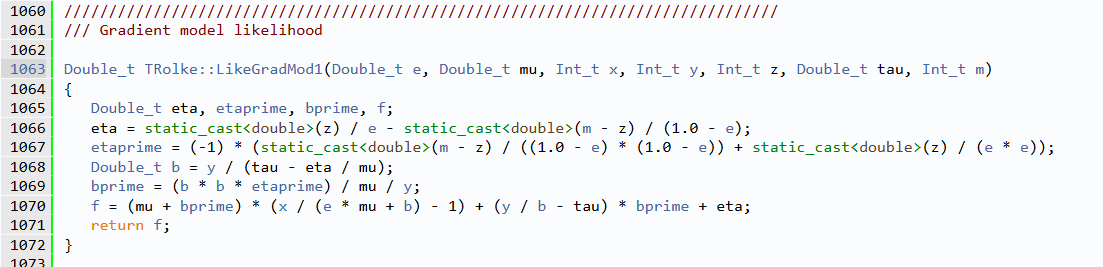
\includegraphics[width=1\textwidth]{graphics/code_with_error.png}};
        \begin{scope} [x={($0.1*(image.south east)$)}, y={($0.1*(image.north west)$)}]


         \draw[line width=0.4mm, red] (0.7, 2.6) rectangle (3.9, 4.1); 
         \draw[red] (3.9, 4.1) ++(0.7, -0.75) node {Error};
         

        \end{scope}
    \end{tikzpicture}
    \caption{Technical implementation of the derivative evaluation.}
    \label{fig:code_with_error}
\end{figure}

The suprema computed by this method are smaller than those obtained using the analytic solution, as will be demonstrated explicitly below.
After correcting this error, the bisection method finds local extrema with respect to $\epsilon$ that concur with the analytic solution; however, in most cases, these are not the desired supremum of the likelihood function.

\section{Implementation of the Fix Based on the Analytic Solution}
There exist different analytic methods for solving a quartic equation. The Ferrari method was chosen due to the relative simplicity of writing the solution in analytic form (see “Summary of Ferrari Method” in \cite{Eq_solve}).
The implementation of the method is given in the listing below. Comparisons of the suprema for different parameters are shown in Figs.~\ref{fig:Rolke_comparsion_0}, \ref{fig:Rolke_comparsion_1}, \ref{fig:Rolke_comparsion_2} (in all plots, the $y$-axis shows $-\sup 2\ln L$ to enable the use of a logarithmic scale).

\begin{figure}[tbph]
   \centering
   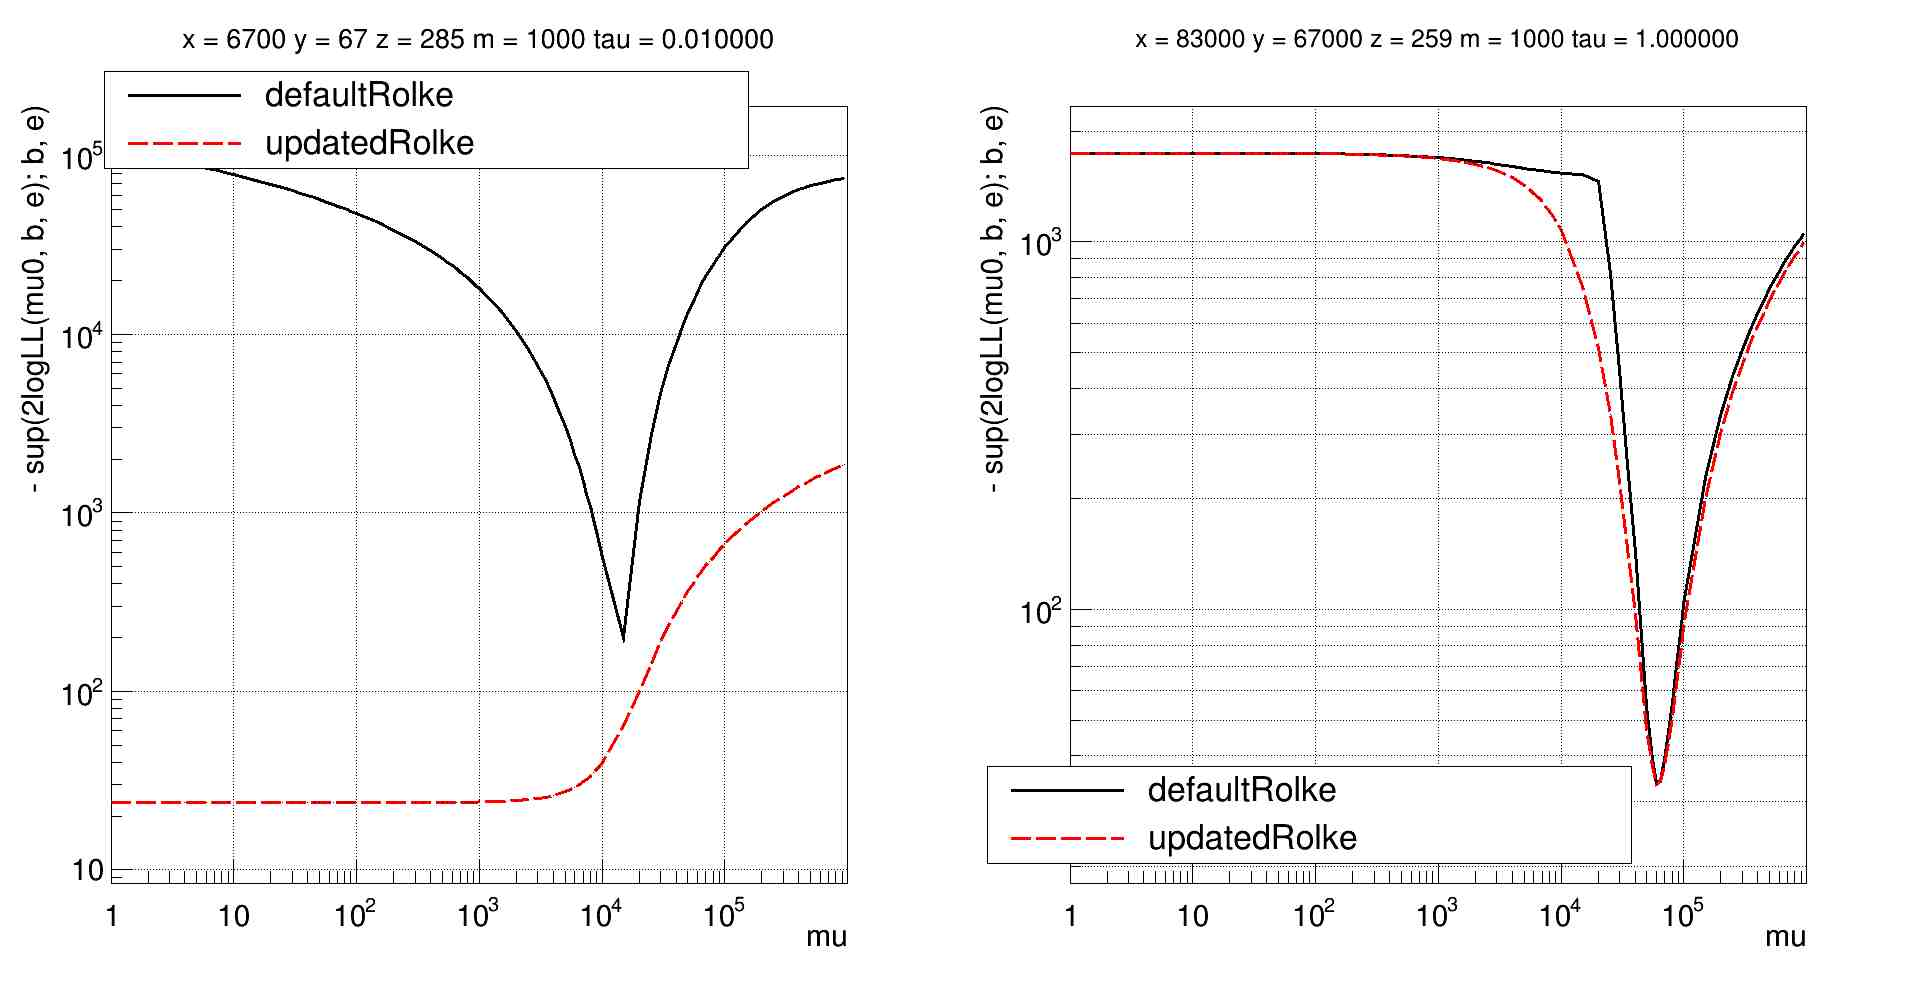
\includegraphics[width=1\textwidth]{graphics/Rolke_comparsion_2_pretty.jpg}
   \caption{Comparison of the suprema obtained with the original and the analytic methods for different parameters.}
   \label{fig:Rolke_comparsion_0}
\end{figure}

\begin{figure}[H]
   \centering
   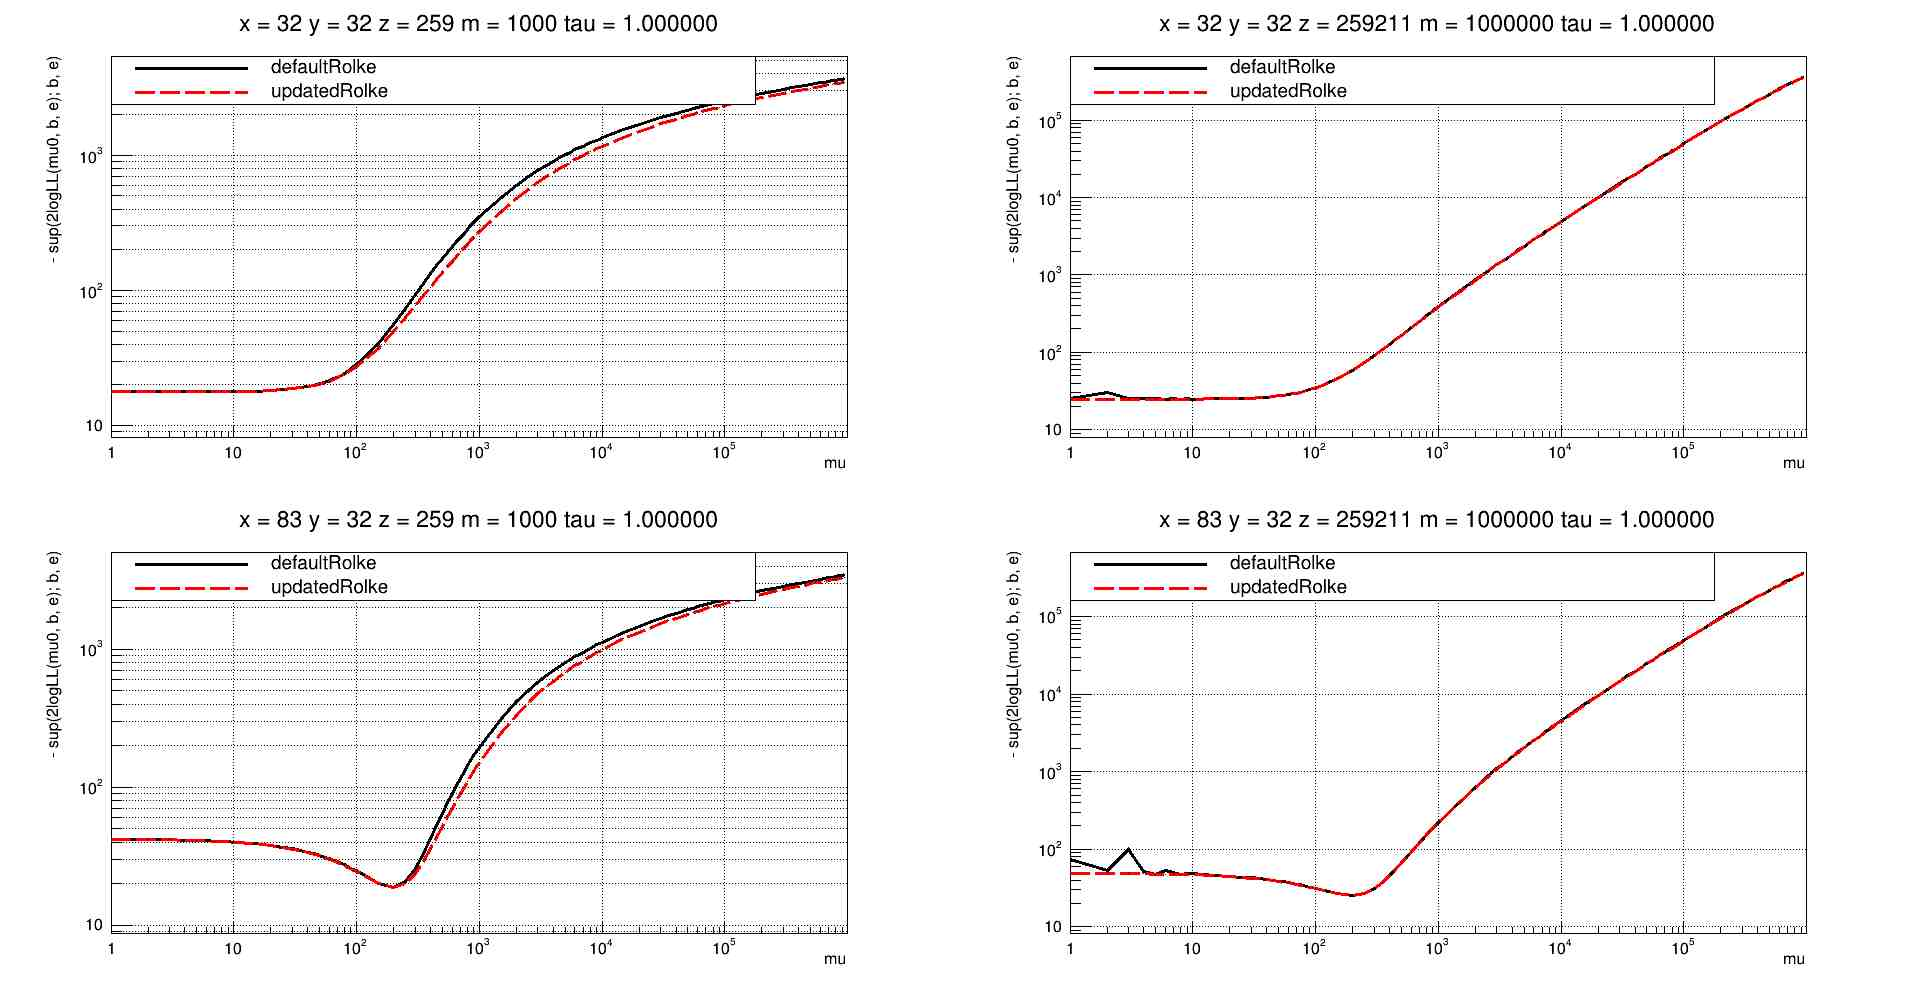
\includegraphics[width=1\textwidth]{graphics/Rolke_comparsion_0_pretty.jpg}
   \caption{Comparison of the suprema obtained with the original and the analytic methods for different parameters.}
   \label{fig:Rolke_comparsion_1}
\end{figure}

\begin{figure}[H]
   \centering
   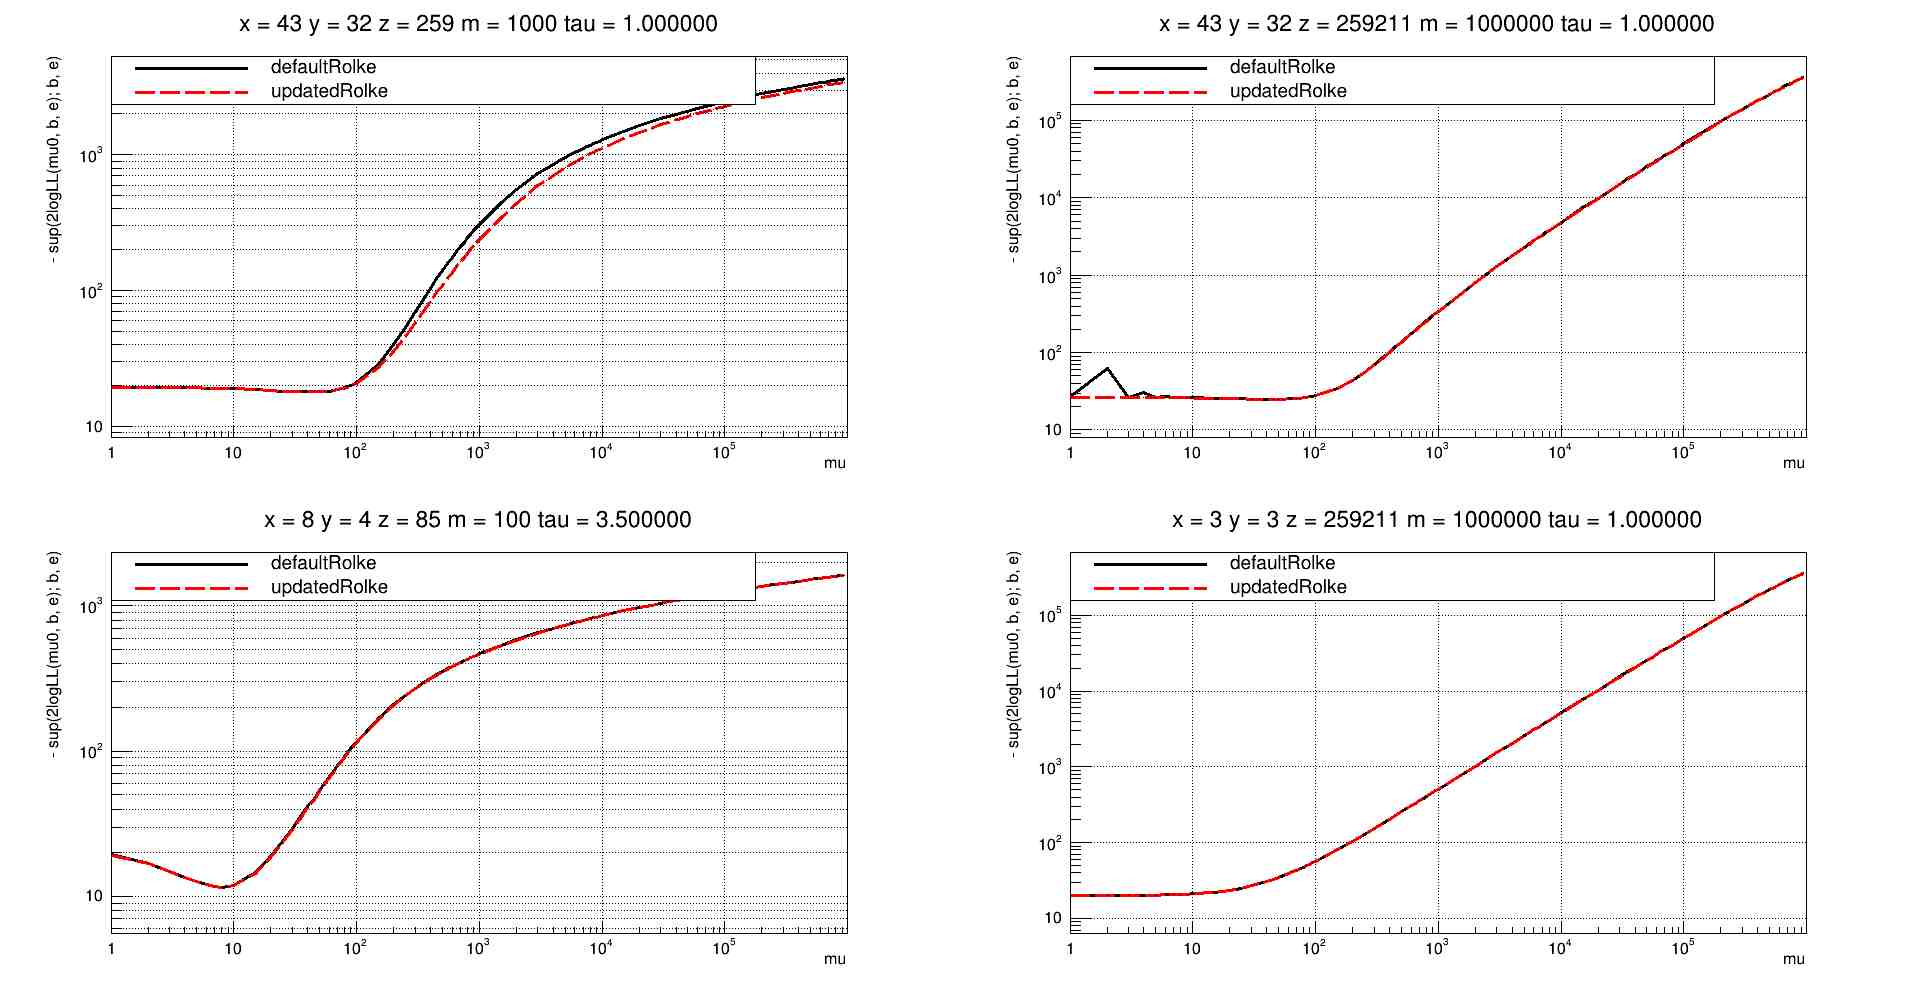
\includegraphics[width=1\textwidth]{graphics/Rolke_comparsion_1_pretty.jpg}
   \caption{Comparison of the suprema obtained with the original and the analytic methods for different parameters.}
   \label{fig:Rolke_comparsion_2}
\end{figure}

It can be seen that the suprema obtained analytically take larger values than the suprema produced by the original method. It is also worth noting the absence of outliers in the analytic solution.

\section{Uncertainties in the Current Analytic Solution}
For some values of $\mu, x, y, z, m, \tau$, all solutions of the system may lie in an unphysical region. The current implementation does not account for this. The question of how this affects the coverage properties of the confidence intervals is not addressed.

\begin{thebibliography}{99}

\bibitem{Rolke_paper}
Rolke W. A., López A. M., Conrad J. Limits and confidence intervals in the presence of nuisance parameters // Nuclear Instruments and Methods in Physics Research Section A: Accelerators, Spectrometers, Detectors and Associated Equipment. – 2005. – Vol. 551. – No. 2–3. – pp. 493–503.

\bibitem{TRolke}
Lundberg J. et al. Limits, discovery and cut optimization for a Poisson process with uncertainty in background and signal efficiency: TRolke 2.0 // Computer Physics Communications. – 2010. – Vol. 181. – No. 3. – pp. 683–686.

\bibitem{ROOT}
ROOT (data analysis framework), https://root.cern/, accessed 2021-02-25

\bibitem{Eq_solve}
\url{https://en.wikipedia.org/wiki/Quartic_equation}

\end{thebibliography}

\newpage

\subsection{Code Listing of the Analytic Implementation for Finding the Supremum}

\begin{lstlisting}[language=C++, basicstyle=\tiny]

void TRolke128_num::ProfLikeMod1Fix(__float128 mu, __float128 &b, __float128 &e, 
      Int_t x, Int_t y, Int_t z, __float128 tau, Int_t m)
{
   __float128 A = - mu * tau * (1.0Q + tau)*(1.0Q + tau);
   __float128 B = mu * (1.0Q + tau) * (- mu * tau * (1.0Q + tau) + 2.0Q * tau * x + y + 
   3.0Q * tau * y + m * (1.0Q + tau));
   __float128 C = mu * (- (x + y) * (tau * x + 2.0Q * y + 3.0Q * tau * y) - 
   m * (1.0Q + tau) * (x + 2.0Q * y) + mu * (1.0Q + tau) * (y + z + tau * (x + 3.0Q * y + z)));
   __float128 D = mu * y * (((__float128) (x + y) * (x + y))  -
    mu * (x + 2.0Q * tau * x + 2.0Q * y + 3.0Q * tau * y + 2.0Q * (1.0Q + tau) * z) + m * (x + y));
   __float128 E = mu * mu * y * y * (x + y + z);

   auto poly4comp = [A, B, C, D, E] (__complex128 b) -> __complex128 {
      __complex128 b_2 = b * b;
      return A * b_2 * b_2 + B * b_2 * b + C * b_2 + D * b + E;
   };

   auto poly4rat = [A, B, C, D, E] (__float128 b) -> __float128 {
      __float128 b_2 = b * b;
      return A * b_2 * b_2 + B * b_2 * b + C * b_2 + D * b + E;
   };

   __float128 A_2 = A * A;
   __float128 B_2 = B * B;

   __float128 alpha = -3.0Q * B_2 / (8.0Q * A_2) + C / A;
   __float128 alpha_2 = alpha * alpha;
   __float128 beta = B_2 * B / (8.0Q * A_2 * A) - B * C / (2.0Q * A_2) + D / A;

   __float128 gamma = - 3.0Q * B_2 * B_2 / (256.0Q * A_2 * A_2) +
    B_2 * C / (16.0Q * A_2 * A) - B * D / (4.0Q * A_2) + E / A; 

   __float128 P = - alpha_2 / 12.0Q - gamma;
   __float128 Q = - alpha_2 * alpha / 108.0Q + alpha * gamma / 3.0Q - beta * beta / 8.0Q;

   __complex128 R = - Q / 2.0Q + csqrtq(Q * Q / 4.0Q + P * P * P / 27.0Q); // taken + sqrt

   __complex128 U = cpowq(R, 1.0Q / 3.0Q);

   __complex128 y_eq =- 5.0Q / 6.0Q * alpha + U - P / (3.0Q * U); // assuming that U !=0;
   __complex128 W = csqrtq(alpha + 2.0Q * y_eq);

   __complex128 back[4]     = {-1.0Q,  -1.0Q, -1.0Q, -1.0Q};
   __complex128 eff[4]      = {10.0Q,  10.0Q, 10.0Q, 10.0Q};
   __float128 minusPlusS[4] = { 1.0Q,   1.0Q, -1.0Q, -1.0Q};
   __float128 minusPlusT[4] = { 1.0Q,  -1.0Q,  1.0Q, -1.0Q};

   __float128 maxLL = (-1.0Q) * FLT128_MAX; 
   __float128 backResult = 0;
   __float128 effResult = 0;

   // loop through signs
   for (int j = 0; j < 4; j ++) {

      back[j] = - B / (4.0Q * A) + (minusPlusS[j] * W + minusPlusT[j] *
       csqrtq(-(3.0Q * alpha + 2.0Q * y_eq + minusPlusS[j] * 2.0Q * beta / W))) / 2.0Q;
      eff[j] = CalcEff(mu, back[j], x, y, z, tau, m);

      __complex128 poly4compVal = poly4comp(back[j]);

      if (crealq(eff[j]) <= 1.0Q && crealq(eff[j]) >= 0.0Q && crealq(back[j]) >= 0.0Q) {
         __float128 currentLL = LikeMod1(mu, crealq(back[j]), crealq(eff[j]), x, y, z, tau, m);
         if (currentLL >= maxLL) {
            backResult = crealq(back[j]);
            effResult = crealq(eff[j]);
            maxLL = currentLL;
            
         } else {
            std::cout << "CurrentLL < maxLL" << std::endl;
         }
         
      } else {
         std::cout << "e or/and b are out of range" << std::endl;
      }

   }

   std::cout << "backResult: " << (double) backResult << " effResult: " << (double) effResult << std::endl;
   b = backResult;
   e = effResult;
}

\end{lstlisting}

\end{document}